\documentclass[15]{article}
\usepackage{graphicx}

\begin{document}

\section{Index}
\begin{enumerate}
\item Project Specification 
\item How to acheieve it 
\item Technolgies
\item Real analysis
\item Tools
\end{enumerate}
\pagebreak 
\section{Project Specification}

\textbf{Aim}: To show simplified math equations on Network Graph\\
\\
\textbf{How to achieve it}
\
\begin{enumerate}

\item User will enter Latex in input box if that latex present in database then will receive Mathml data as AST from db Directly and need to represent on graph


\item If latex is not present in database then it will convert to Mathml first then that Mathml
Is simplified to its final equation using parser in return we will get AST of Mathml that we have to display those as Node and edges where Nodes represent mathml and edges represent relations between each equation.

\item If latex is not present in db then we have to follow step2 and need to store data in db
\end{enumerate}

\subsection*{Technologies}


\begin{enumerate}
\item Sigmajs/D3 js
\item NeoSigma4j/Postgress
\item Ocaml 
   
\end{enumerate}

\subsection*{Terminologies}

\begin{enumerate}
\item Mathml: Mathml is an XML to represent latex or Mathematical formulas  on browsers
\item AST: AST stand for Abstract Syntax Tree, is  a tree type representation of source code
\item Latex: LaTeX, computer programming language used for typesetting technical documents. 


\end{enumerate}



\subsection*{Tools/Libraries}

\begin{enumerate}
\item Lexer \&\ Parser's:  Parser will convert equations into ast and parser can simplify equations
Matml converter: Lib/script which convert latex or equations in Mathml.

\item Theorem Prover's: Example HOL Light

\end{enumerate}
\pagebreak

\section{Real analysis}

\paragraph{Real Number}
A real number is any positive or negative number. This includes all integers and all rational and irrational numbers. Rational numbers may be expressed as a fraction (such as $\frac{7}{8}$) and irrational numbers may be expressed by an infinite decimal representation $ (3.1415926535...)$

In general, all the arithmetic operations can be performed on these numbers and they can be represented in the number line, also. At the same time, the imaginary numbers are the un-real numbers, which cannot be expressed in the number line and is commonly used to represent a complex number. 
\\
\\
The set of real numbers are consist of different categories, such as, natural and whole numbers, rational and irrational numbers and integers.


\paragraph{Real analysis} Real analysis is a field in mathematics that focuses on the properties of real numbers, sequences and functions
\\
\\
Study of Real number system:
\begin{enumerate}

\item Natural Number: 1 to infinte also called countuing numbers
 Whole Numbers: 0, 1,2 ... to infinite
\item Intgers:  negative infinite .... 0.... Poistive infinite 
\item Rational number:  denoted By Q = $\frac{p}{q}$ where \item q is not equal to zero and p,q must be integers and p,q must not have any common factors
\item Irratiional number: Which cannot be represnted on p/q form like root 2

\end{enumerate}

\paragraph{Cauchy Sequence }
A sequence is said to be a cauchy sequence  for every epsilon greater than zero.There is a positive integer $m          m, n > N then |am- an| < ε. \forall  m>n$ \\
\\
First we will construct Natural Numbers:
\\
Constructing Real numbers with Peano’s Axiom
\
\vspace{5mm} %5mm vertical space

\textbf{Axioms:}
\\*
\begin{enumerate}
\item There exist a natural number 1
\item If a is a natural number, then its successor  s(a) = a+1 is also a natural number.
\item 1 is not the successor is any natural number
\item If two numbers have the same successor then they must be the same number.
\item Given a set S, if 1 belongs to S and contains the successor of any number in S then S must contain all of the natural numbers.\\
\end{enumerate}

\textbf{Some basic definition:}

\textbf{Least element}:  Let A is subset of Q where Q is a set of all Rational number, r  Q then r is said to be least element of A only if
$$r {\in} A:r {\leq x} ,{\forall} x {\in} A$$. \\   
\\
\\
\textbf{Largest element:}  Let A is subset of Q where Q is a set of all Rational number, $ u {\in} Q $ then u is said to be Largest element of A only if
$$u {\in} A
u {\geq} x, \forall x \in A $$
\\
\\*
(This definition is in my own words may be not like standard definition)\\
\\
\textbf{Dedekind Cuts:}  Since the set of rational is an ordered field so  we can arrange this set of rational number Q on number line. Suppose we mark a cut P on that number line such that it divides number line in two parts or in two sub set of Q.
\\
What we will have after dividing the number line:
\begin{enumerate}
\item There will be two part one on left hand “L” called lower class element and other on Right hand side “U” called Upper class elements.

\item Lower class “L” elements are smaller that Upper class elements “U”.

\item There are two possibilities for cut “P”. It could be Rational number or irrational number.

\item If P is irrational number then all rational either belongs to “L” or belongs “U” and P itself become the largest element of U.

\item If cut P is a rational number then means P is in the form of p/q
Then P belongs to “U”. Means P will be element of Right hand set
\pagebreak

\textbf{Standard Definition from above explanation}
\\
A Dedekind cut x = (L, U) in Q is a pair of subset L,U of Q satisfying the following condition
\begin{enumerate}
\item $L \cup U$ = Q ,  $L \cap U$ = {}, L and U are non empty sets
\item If l belongs L and u belongs U then $l<u$
\item L will not have the largest element 


\end{enumerate}




\end{enumerate}


\section{HOL Light}
Referencing link for HOL LIGHT:   https://github.com/jrh13/hol-light/
\\
\\
Basic
Author: John Harrison 
\\
\\
\\
\\
HOL Light is a computer program to help users prove interesting mathematical theorems completely formally in higher order logic. It sets a very exacting standard of correctness, but provides a number of automated tools and pre-proved mathematical theorems (e.g. about arithmetic, basic set theory and real analysis)
\pagebreak

\textbf{HOL Light Basics}

\begin{enumerate}

\item \textbf{Terms}
\\
Terms are like  strings  in  that  they  are  manipulated  purely  as  symbolic  expressions.

$$ {`}x+1{`} $$   

\item \textbf{Types}
\\
A key feature of HOL is that every term has a well-definedtype.  Roughly speaking,the type indicates what kind of mathematical object the term represents (a number, aset, a function, etc.)  The possible types of terms are represented using another sym-bolic datatypeholtype, and these will similarly be automatically parsed and printedwithin backquotes with a colon as the first character.


\begin{verbatim}  type_of ‘1‘;;
val it : hol_type = ‘:num‘# 
\end{verbatim}

\begin{verbatim} type_of ‘x + 1 < x + 2‘;;
val it : hol_type = ‘:bool‘
\end{verbatim}


\item \textbf{Theorems}\\
 A specialtypethm(‘theorem’) is used for formulas


\begin{verbatim}
# REFL ‘x:real‘;;
val it : thm = |- x = x 
# let th1 = REFL ‘x + 1‘;;
val th1 : thm = |- x + 1 = x + 1
\end{verbatim}
\end{enumerate}


HOL Light Code 

File name Lib.ml\\

\textbf{map}
\begin{figure}

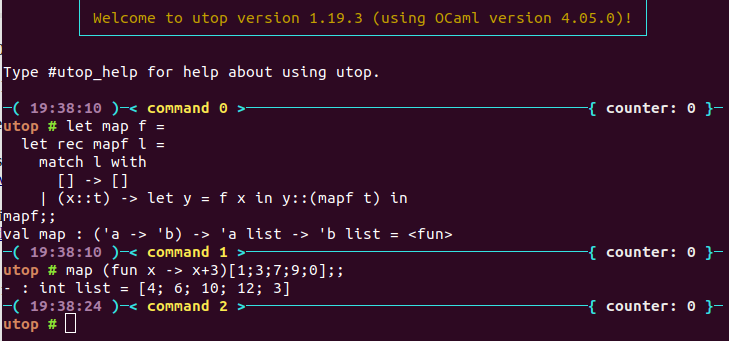
\includegraphics[scale = .5]{images/image4.png}
Takes funtion and list and appiles function to each element of list:
\\
\\

\textbf{last}
\begin{figure}
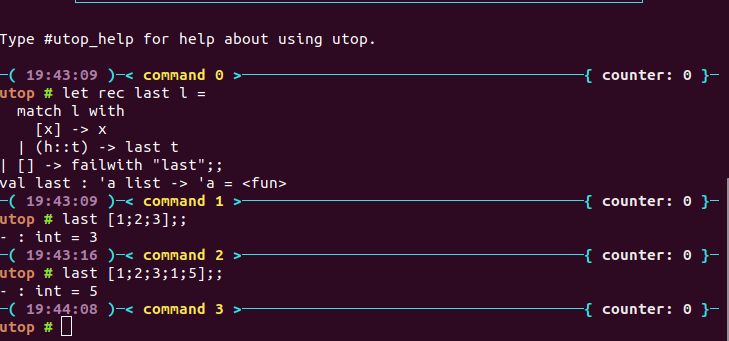
\includegraphics[scale = .5]{images/image10.png}
\\
\\
This functions takes List and return last element of the list
and if list is empty then exception: Failure "last".\\
\\
\end{figure}
\\
\textbf{butlast}\\
\\
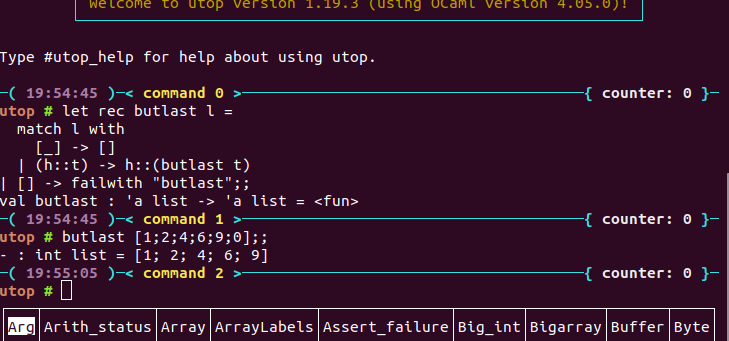
\includegraphics{images/image9.png}
\\
as you can see in screenshot this function gives list except last element.\\
butlast [1;2;4;6;9;0];; \\
- : int list = [1; 2; 4; 6; 9] \\
\\
\\
\textbf{el}\\
\\
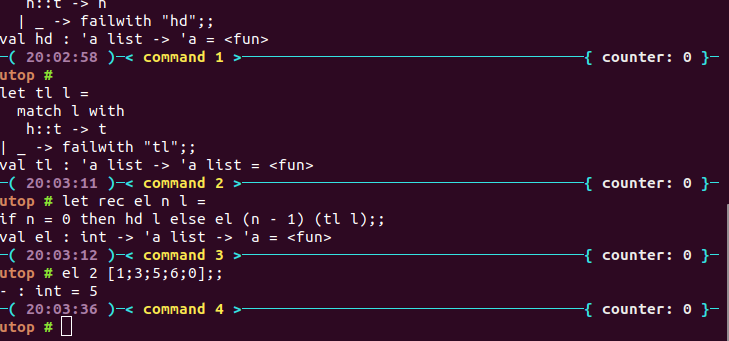
\includegraphics[scale = .5]{images/image8.png}
\\
el function gives specfied element from list
Consist of two other function hd , tl  specifies in lib.ml \\
\\
\\
\textbf{rev}\\
\\
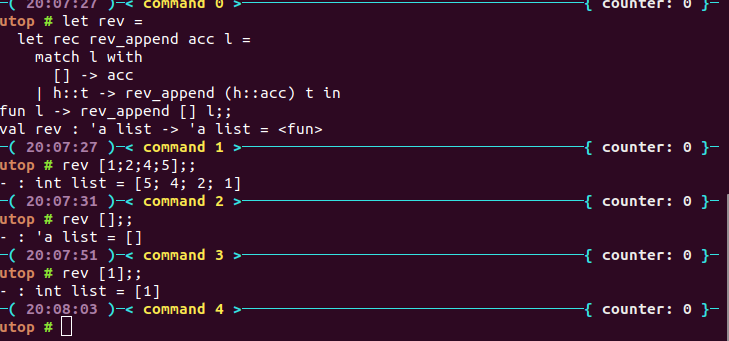
\includegraphics[scale = .5]{images/image5.png}
\\
\\
return reversed list\\
\\
\textbf{map2}
\\
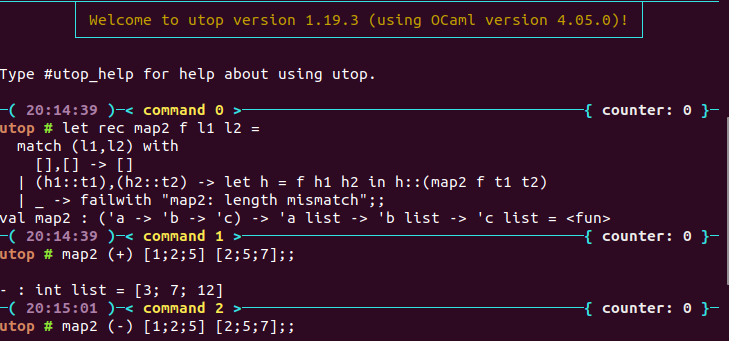
\includegraphics[scale = .5]{images/image3.png}
\\
maps2 take two list and function and gives new list\\
map2 f ([x1;...;xn],[y1;...;yn]) returns [f(x1,y1);...;f(xn,yn)].\\
\\
\textbf{funpow}
\\
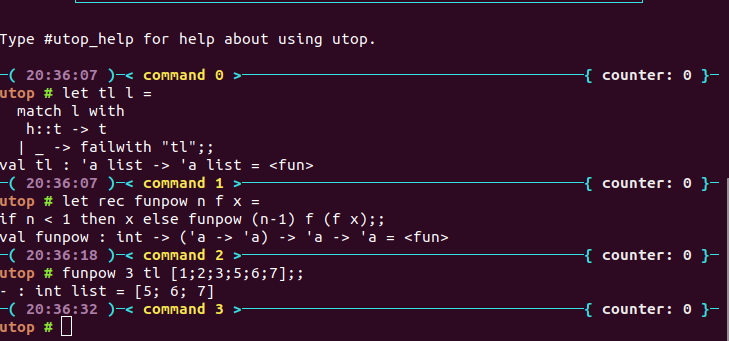
\includegraphics[scale = .5]{images/image11.png}
\\
This function takes 3 argument: int -> ('a -> 'a) -> 'a -> 'a = <fun>\\
how many times n a function f applies to x
\\
\\
\textbf{itlist}
\\
\\
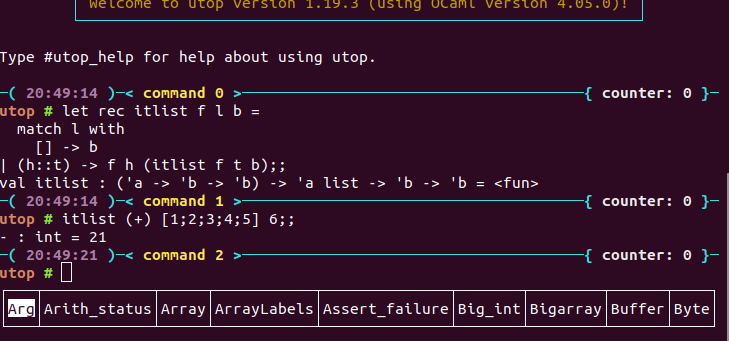
\includegraphics[scale = .5]{images/image2.png}
\\
\\
This function applies function f to adjacent element of list\\
\\
\\
\textbf{SET OPERATIONS ON LIST:
}\\
\\
\textbf{mem}\\
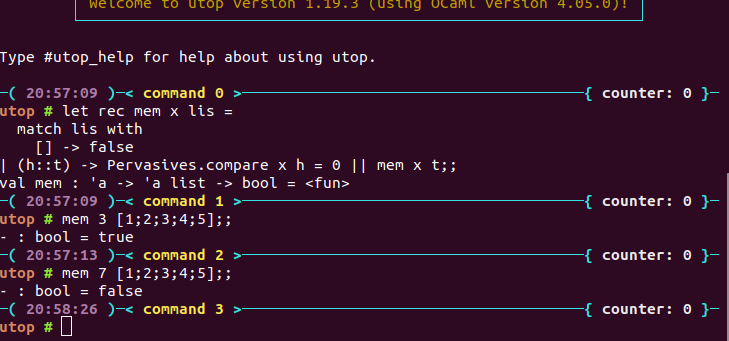
\includegraphics[scale = .5]{images/image7.png}
\\
mem is a boolen type function\\
returns true if given element is present in list else return false\\
\\
\\
\textbf{Insert}\\
\\
\\
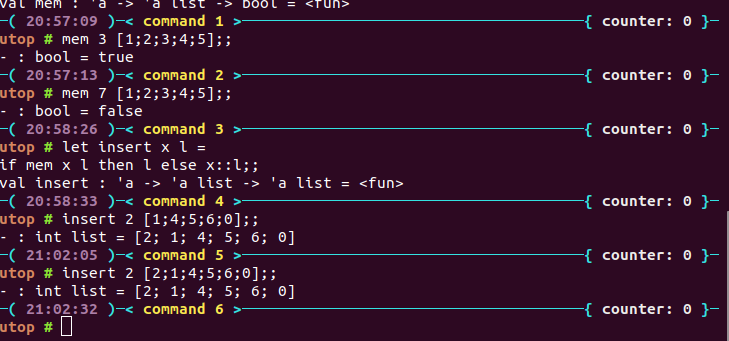
\includegraphics[scale = .5]{images/image12.png}
\\
\\
insert function checks element is present in list if not the insert that element in that list\\
\\
\\
\textbf{union}\\
\\
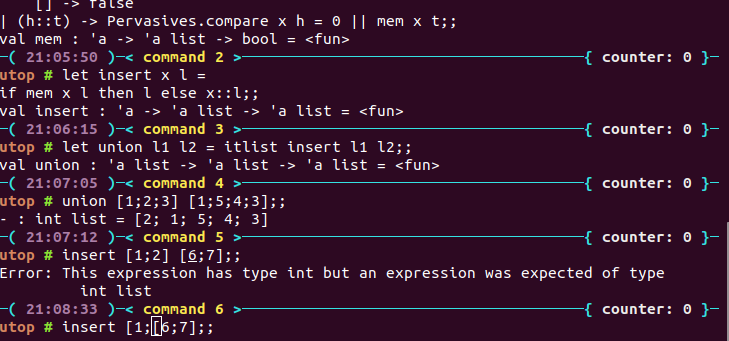
\includegraphics[scale = .5]{images/image6.png}
\\
\\
Union returns a list consisting of the elements of l1 not already in l2 concatenated with l2\\

\pagebreak

\textbf{13-01-2020}\\
\\
Worked on compiling an \texttt{incr\_dom} dom file with HOL Light and intro.ml.
First checked how to compile \texttt{incr\_dom} with file HOL light and use input from
web to HOL light and print result on web.\\
\\
As hol light consist of lots of files and so currently i dont know how
pass web input to Hol light.\\
\\
In order to work with hol light theorem prover first i have tested how to use
\texttt{incr\_dom}  with intro.ml\\
\\
\\
Used files:\\
\\
Intro.ml from sml handbook\\
\texttt{Input\_text} example code from \texttt{incr\_dom}
\\
code line: app.ml 13,20,75

Issue Faced:
\texttt{incr\_dom} examples are not compiling with Hol light
\\ 
 unused variables issue when compiling with inro.ml
 \\
 Solutiton worked
\\ 
\begin{verbatim}

dune  build example/text_input/{main.bc.js,index.html} --profile release
\end{verbatim}
\\
Use above command to build project


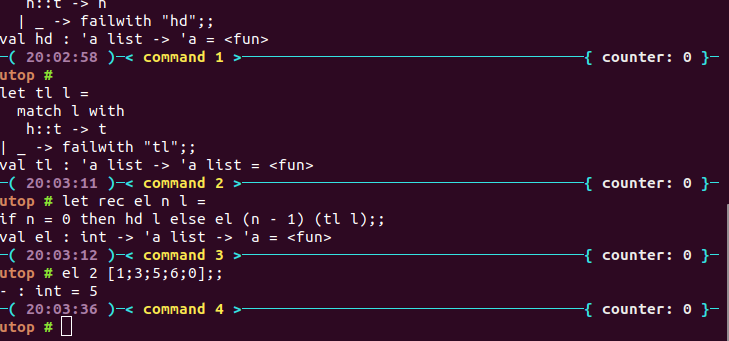
\includegraphics[scale = .5]{images/image8.png}

	
\end{document}

